\documentclass[aspectratio=169,hyperref={unicode}]{beamer}

\usetheme{Szeged}
\usecolortheme{beaver}
\usepackage{fontspec}
\usepackage{xcolor}
\usepackage{ulem}
\usepackage{hyperref}
\usepackage[german]{babel}
\usepackage{tikz}
\usetikzlibrary{positioning}

\title{A Gentle Introduction to Programming}
\author{Erik Zeiner}
\institute{Fachschaft General \& Computational Linguistics\\ \textbf{University of Tübingen}}
\date{WS 2024/25 \\ Pre-course}
\begin{document}
\frame{\titlepage}
\begin{frame}{What is programming?}

\begin{center}
	\Large\textbf{Providing instructions on how to perform a task}
\end{center}



\begin{itemize}
	\item This can take many forms; just look at the history of computers!
	\item Nowadays, we are usually talking about computer programming - writing code
\end{itemize}
	
\end{frame}
\begin{frame}{Programming vs. Algorithms}
	
\begin{block}{Programming}
	A sequence of instructions used to tell the computer to perform a task.
\end{block}
	
\begin{block}{Algorithm}
	A sequence of steps used to solve a specific problem.
\end{block}
 
\vfill

Within the scope of programming, you will be both:
\begin{itemize}
	\item using existing algorithms and
	\item designing your own
\end{itemize}

\end{frame}

\begin{frame}{How does the computer follow your instructions?}
\begin{figure}
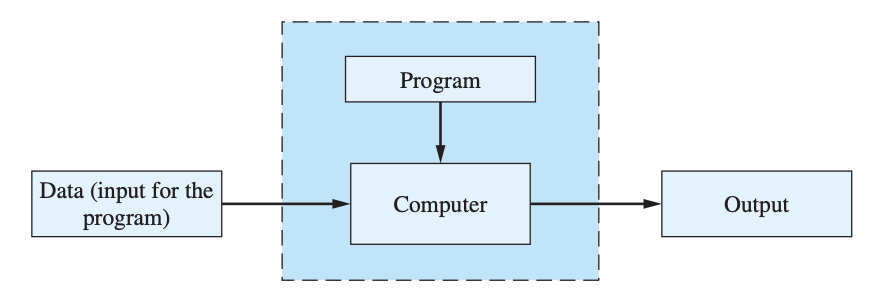
\includegraphics[width=\linewidth]{Screenshot.png}  
\caption{From 'Java: An Introduction to Problem Solving \& Programming'}
\end{figure}
\end{frame}

\begin{frame}{How does the computer understand your code?}
  \begin{tikzpicture}
    % Rectangle 1
    \node [draw, rectangle,align=left] (rect1) {\textbf{Source code} \\
    A text file with series of instructions\\
    Written in a high-level programming language\\ Understandable by humans};

    \node [draw, rectangle, align=left, below=1cm of rect1] (rect2) {\textbf{Compiler or Interpreter} \\ High-level lang. $\rightarrow$ Low-level lang.};

    \node [draw, rectangle, align = left, right=1 cm of rect2] (rect3) {\textbf{Machine code}\\A file with executable code \\
    Translated into a low-level language\\ Understandable by computers};

    % Arrows
    \draw[->] (rect1) -- (rect2);
    \draw[->] (rect2) -- (rect3);
  \end{tikzpicture}
\end{frame}

\begin{frame}{How do you actually go about writing a program?}

\begin{center}
	\Large\textbf{Theoretical part}
\end{center}
When faced with a real-world problem we want to solve:
\begin{itemize}
	\item Analyse the problem - understand it as a series of discrete logical steps
	\item Design a way to solve it - again, thinking in steps\\This could be done on paper; it's not about coding, it's about thinking!
	\item Instruct the computer to follow your solution
\end{itemize}

\end{frame}

\begin{frame}{How do you actually go about writing a program?}

\begin{center}
	\Large\textbf{Practical part}
\end{center}
\begin{enumerate}
	\item \textbf{Write code} - \textit{it's just plaintext files}\\ text editors provide helpful tools and features for writing code
	\item \textbf{Run \& Test code} - text files interpreted/compiled and instructions executed\\ Use the command line to tell the computer to run the source file	\item \textbf{Debug code} - find and correct errors\\ manually or with a debugger
 
\end{enumerate}
\textbf{Repeat 1. - 3.}

\begin{itemize}
	\item \textbf{Tools:} countless apps, workflows, and ways of writing code - personal preferences + imposed requirements\\
	\textbf{IDEs} - write, run, and debug in one app
\end{itemize}

\end{frame}
\begin{frame}{How does one choose a programming language?}
\begin{itemize}
	\item Personal preference/knowledge
	\item Imposed requirements - platform, project, group, or a company standardisation
	\item Advantages - use-case, speed, available libraries/packages,... 
\end{itemize}

\begin{center}\textbf{Concepts and skills are highly transferable from one language to another}\\ knowing any programming language means others will be easier to pick up\end{center}

\end{frame}
\begin{frame}{Java}
\textbf{Classes you will use it in include: DSA I, DSA II}

\begin{columns}
	\begin{column}{0.3\linewidth}
	\begin{itemize}
		\item Fast
		\item Compiled
		\item Platform independent
		\item Object oriented
		\item Quite in-demand by employers
		\item A tad wordy
	\end{itemize}
	\end{column}

	\begin{column}{0.7\linewidth}
	\begin{center}
			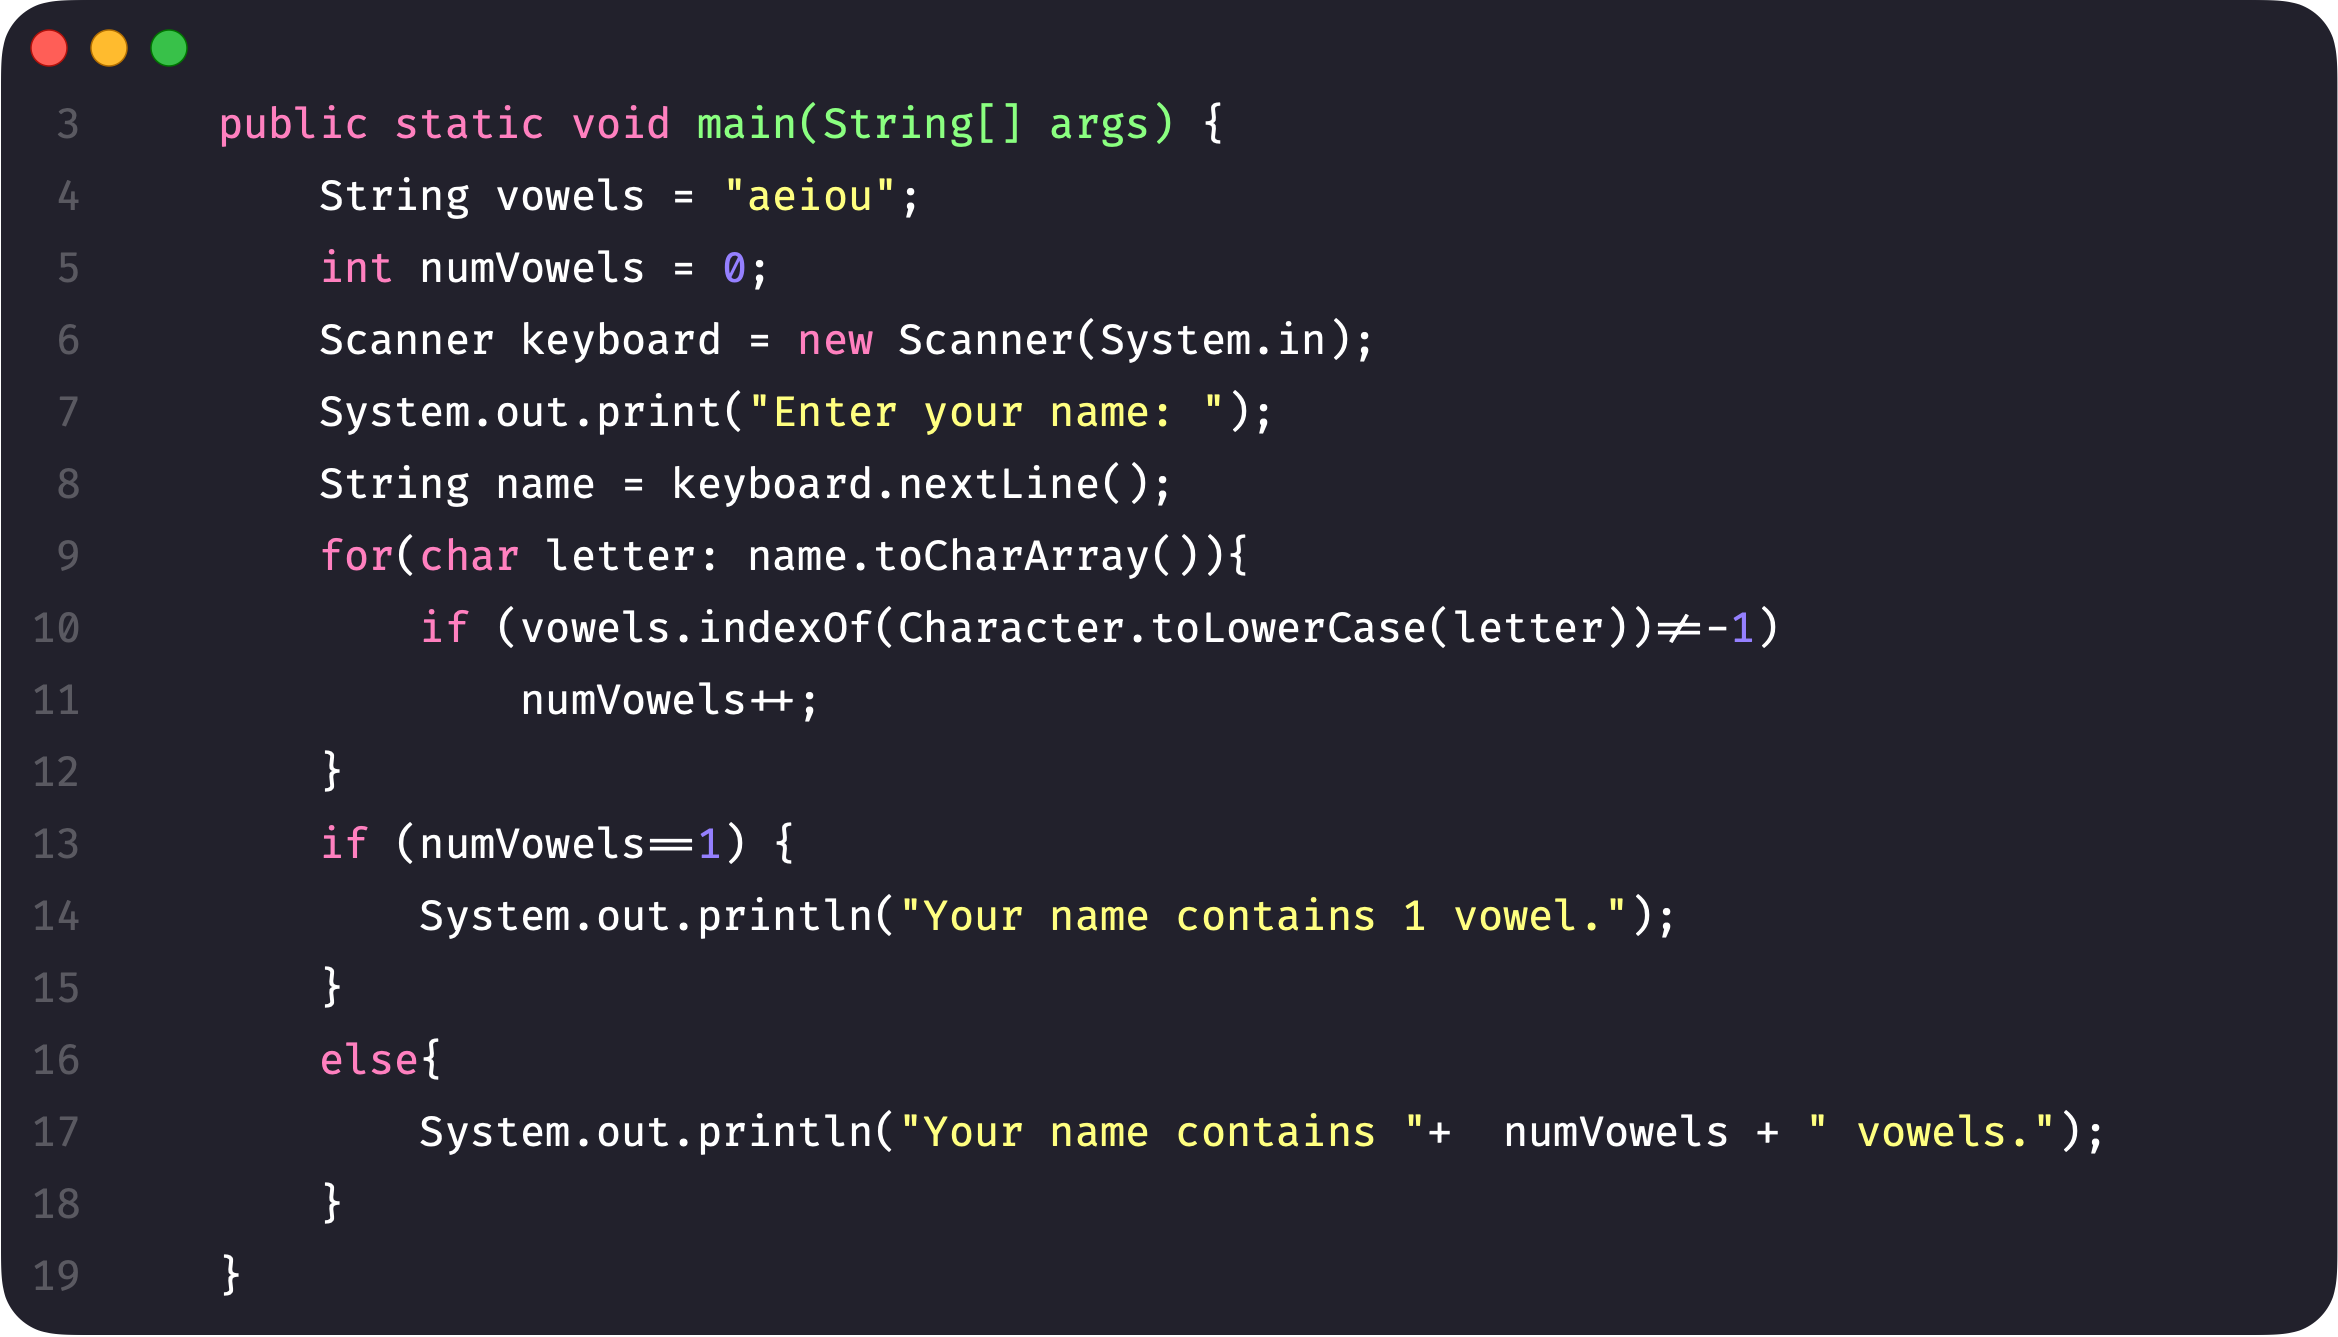
\includegraphics[scale=0.117]{java.png}
	\end{center}
	\end{column}
\end{columns}

\end{frame}

\begin{frame}{Python}
\textbf{Classes you will use it in include: Programming and Data Analysis, DSA III}

\begin{columns}
	\begin{column}{0.3\linewidth}
	\begin{itemize}
		\item Not as fast but more versatile
		\item Interpreted
		\item Platform independent
		\item Object oriented
		\item Quite in-demand by employers
		\item Simpler Syntax
	\end{itemize}
	\end{column}

	\begin{column}{0.7\linewidth}
	\begin{center}
			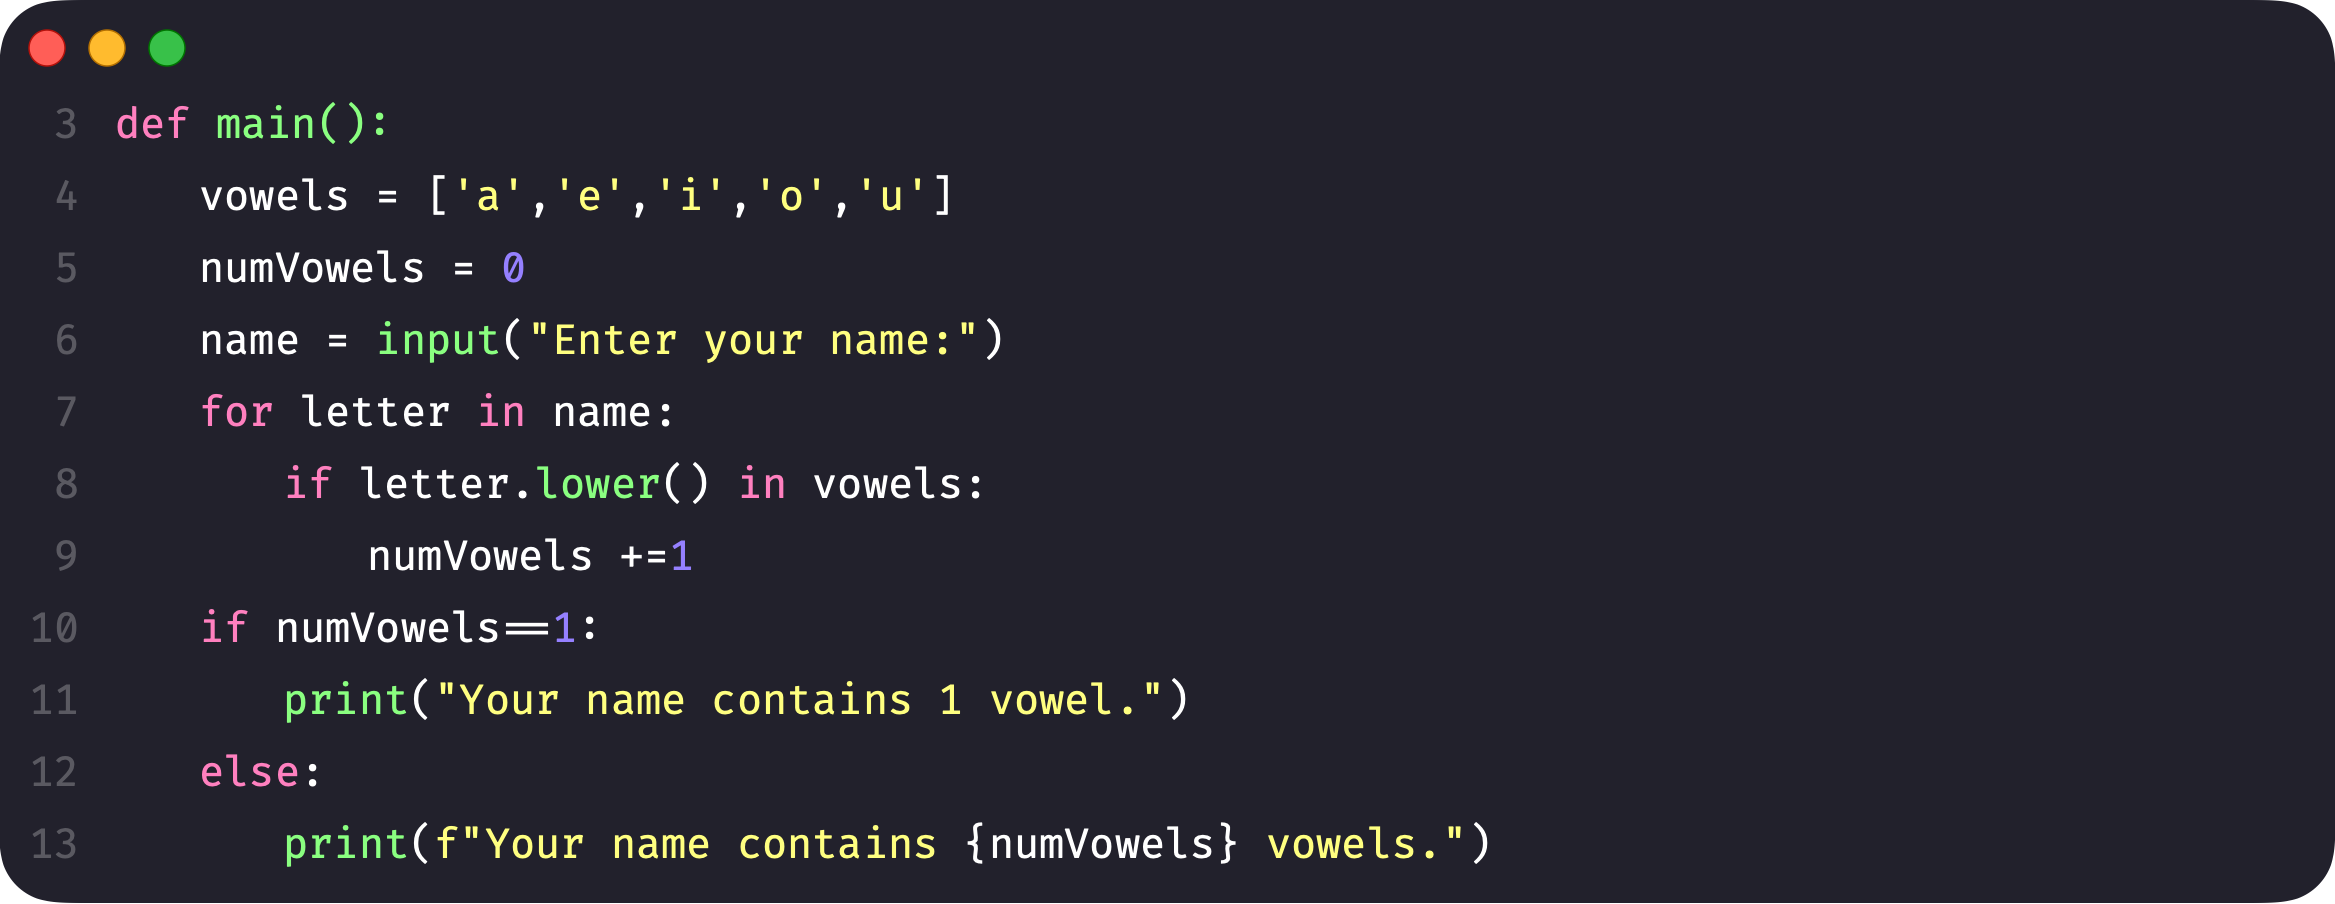
\includegraphics[scale=0.117]{python.png}
	\end{center}
	\end{column}
\end{columns}
\end{frame}

\begin{frame}
\begin{center}

\begin{minipage}{0.4\textwidth}
\centering
    
\includegraphics[width=0.5\textwidth]{../QRqa.png}
  \end{minipage}
  \hfill
  \begin{minipage}{0.4\textwidth}
  \centering
    
\includegraphics[width=0.5\textwidth]{../QRweb.png}
  \end{minipage}
\end{center}
\end{frame}

\end{document}